% --------------------------------------
% Document Class
% --------------------------------------
\documentclass[a4paper,11pt]{article}
% --------------------------------------



% --------------------------------------
% Use Package
% --------------------------------------


\usepackage[francais]{babel}
%\usepackage{ucs}
\usepackage[utf8]{inputenc}
\usepackage[T1]{fontenc}

\usepackage{makeidx}
\usepackage{color}
\usepackage{graphicx}
\usepackage{float}
\usepackage[hidelinks]{hyperref} 
\usepackage{geometry}
%\usepackage{lastpage}
%\usepackage{marginnote}
\usepackage{fancyhdr}
%\usepackage{titlesec}
%\usepackage{framed}
\usepackage{amsmath}
\usepackage{empheq}
\usepackage{array}
\usepackage{multicol}
%\usepackage{adjustbox}

% insert code
\usepackage{listings}

% define our color
\usepackage{xcolor}

% code color
\definecolor{ligthyellow}{RGB}{250,247,220}
\definecolor{darkblue}{RGB}{5,10,85}
\definecolor{ligthblue}{RGB}{1,147,128}
\definecolor{darkgreen}{RGB}{8,120,51}
\definecolor{darkred}{RGB}{160,0,0}

% other color
\definecolor{ivi}{RGB}{141,107,185}


\lstset{
    language=Scilab,
    captionpos=b,
    extendedchars=true,
    frame=lines,
    numbers=left,
    numberstyle=\tiny,
    numbersep=5pt,
    keepspaces=true,
    breaklines=true,
    showspaces=false,
    showstringspaces=false,
    breakatwhitespace=false,
    stepnumber=1,
    showtabs=false,
    tabsize=3,
    basicstyle=\small\ttfamily,
    backgroundcolor=\color{ligthyellow},
    keywordstyle=\color{ligthblue},
    morekeywords={include, printf, uchar},
    identifierstyle=\color{darkblue},
    commentstyle=\color{darkgreen},
    stringstyle=\color{darkred},
}


% --------------------------------------



% --------------------------------------
% Page setting
% --------------------------------------
%\pagestyle{empty}
\setlength{\headheight}{15pt}

\setcounter{secnumdepth}{3}
\setcounter{tocdepth}{2}

\makeatletter
\@addtoreset{chapter}{part}
\makeatother 

\hypersetup{         % parametrage des hyperliens
  colorlinks=true,      % colorise les liens
  breaklinks=true,      % permet les retours à la ligne pour les liens trop longs
  urlcolor= blue,       % couleur des hyperliens
  linkcolor= black,     % couleur des liens internes aux documents (index, figures, tableaux, equations,...)
  citecolor= green      % couleur des liens vers les references bibliographiques
}

% --------------------------------------

% --------------------------------------
% Information
% --------------------------------------
\title{Compte-rendu TP4 TI : Transformation ponctuelle}
\author{Elliot VANEGUE et Gaëtan DEFLANDRE}
% --------------------------------------

\definecolor{myColor}{rgb}{0.5, 0.1, 0.75}

% --------------------------------------
% Begin content
% --------------------------------------
\begin{document}

% Set language to english
  \selectlanguage{francais}

  % Start the page counting
  \pagenumbering{arabic}

  \maketitle
  
  \mbox{}
  \newpage
  \clearpage
  
  \section*{Introduction}
  Lors de ce TP, nous avons travaillé avec l'outil ImageJ dans le but de manipuler des images
  à l'aide de macros. Nous avons analysé les histogrammes de niveaux de gris et mis en 
  évidence certaines opérations possibles sur ces derniers. Ainsi, nous montrerons que ces
  opérations sont souvent associées avec une LUT\footnote{Look Up Table}.

  \section{Extension de dynamique de l'histogramme}
  Pour commencer, nous avons écrit une macro permettant de récupérer les niveaux de gris minimum et 
  maximum d'une image dans le but de les modifier afin d'avoir une dynamique de gris allant de 
  0 à 255. Pour cela nous avons appliqué la transformation linéaire suivante : 
  \begin{align*}
   round\left(\frac{255 * pixel(i,j) - min}{max - min}\right)
  \end{align*}

  Dans cette formule, la fonction round permet d'arrondir le résultat à l'entier le plus proche.
  En effectuant ce calcul sur chaque pixel, nous obtenons les résultats suivants :\\
  
  \begin{tabular}{|c|c|c|c|}
   \hline
   image départ & histogramme & image étendue & histogramme\\
   \hline
   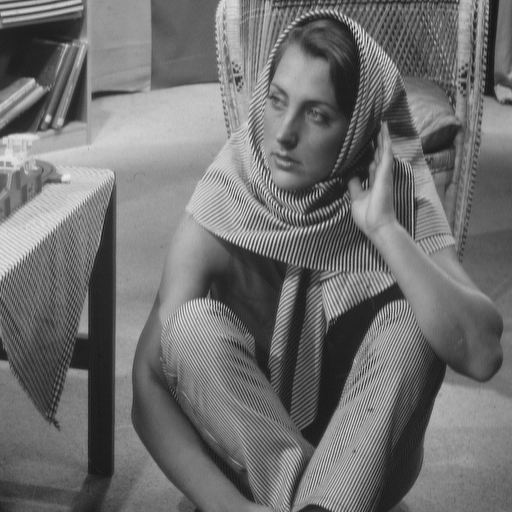
\includegraphics[width=3cm]{barb.png} & 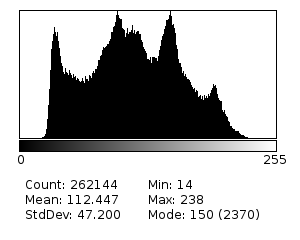
\includegraphics[width=3cm]{../histo/image/hist_barb.png} & 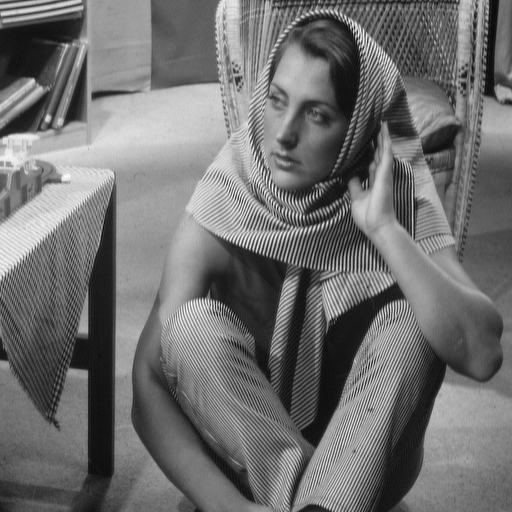
\includegraphics[width=3cm]{../res/barbQ1.png} & 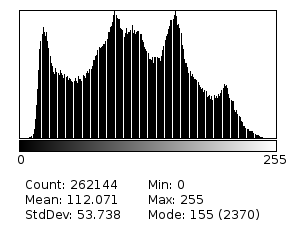
\includegraphics[width=3cm]{../histo/resultat/hist_barbQ1.png}\\
   \hline
   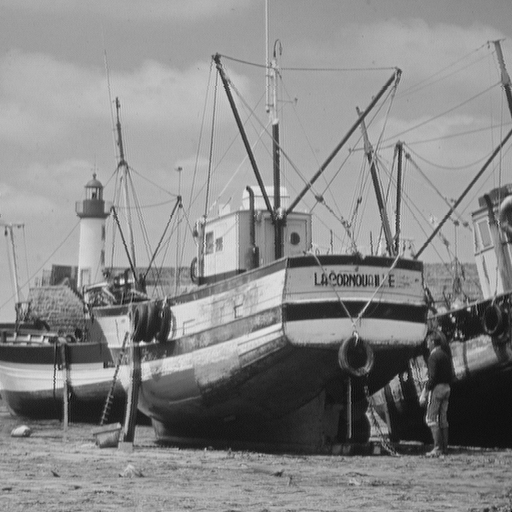
\includegraphics[width=3cm]{boat.png} & 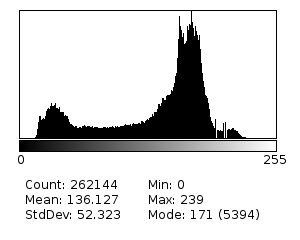
\includegraphics[width=3cm]{../histo/image/hist_boat.png} & 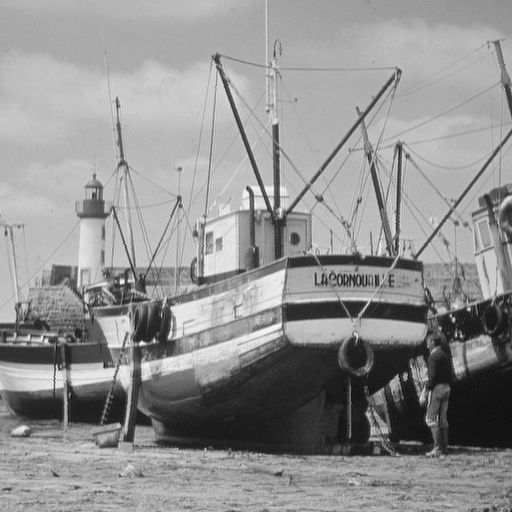
\includegraphics[width=3cm]{../res/boatQ1.png} & 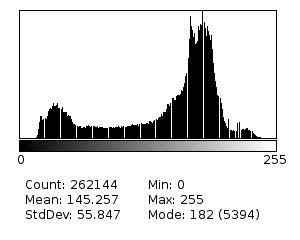
\includegraphics[width=3cm]{../histo/resultat/hist_boatQ1.png}\\
   \hline
   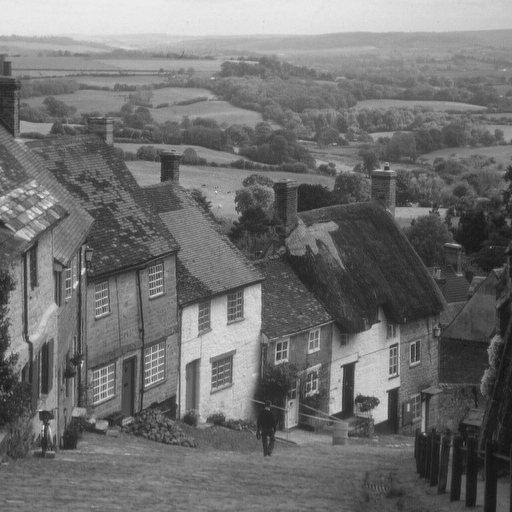
\includegraphics[width=3cm]{goldhill.png} & 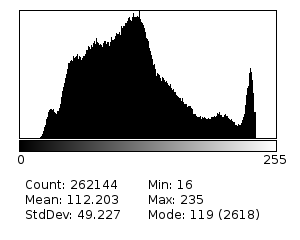
\includegraphics[width=3cm]{../histo/image/hist_goldhill.png} & 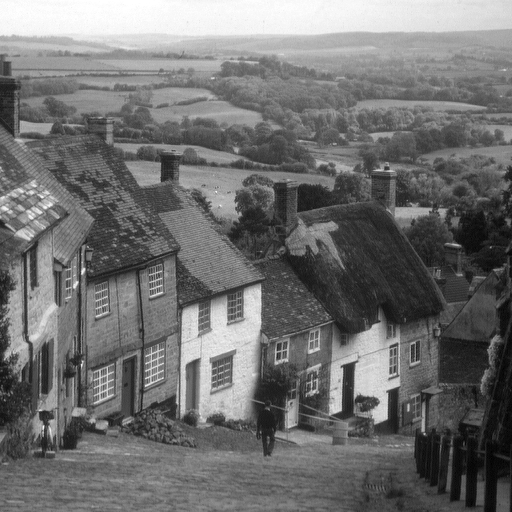
\includegraphics[width=3cm]{../res/goldhillQ1.png} & 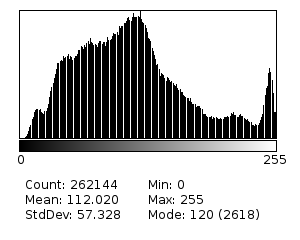
\includegraphics[width=3cm]{../histo/resultat/hist_goldhillQ1.png}\\
   \hline
  \end{tabular}
  
  \newpage
  
  \begin{tabular}{|c|c|c|c|} 
   \hline
   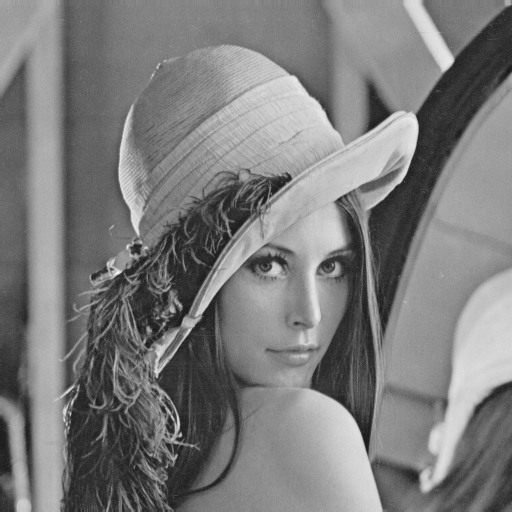
\includegraphics[width=3cm]{lena512.png} & 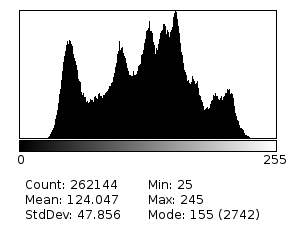
\includegraphics[width=3cm]{../histo/image/hist_lena512.png} & 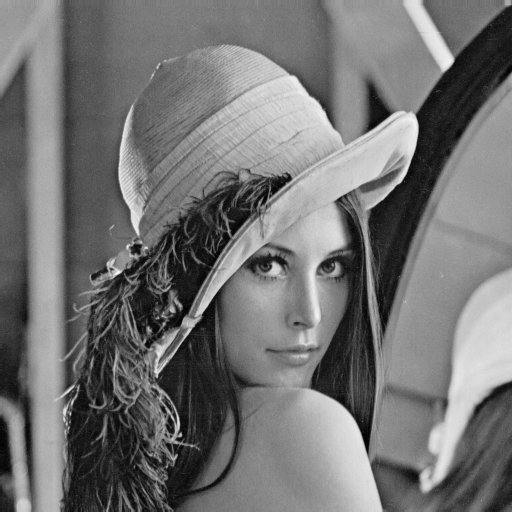
\includegraphics[width=3cm]{../res/lena512Q1.png} & 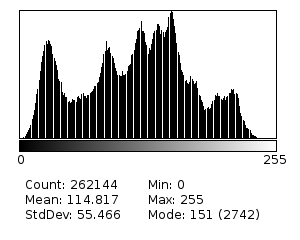
\includegraphics[width=3cm]{../histo/resultat/hist_lena512Q1.png}\\
   \hline
   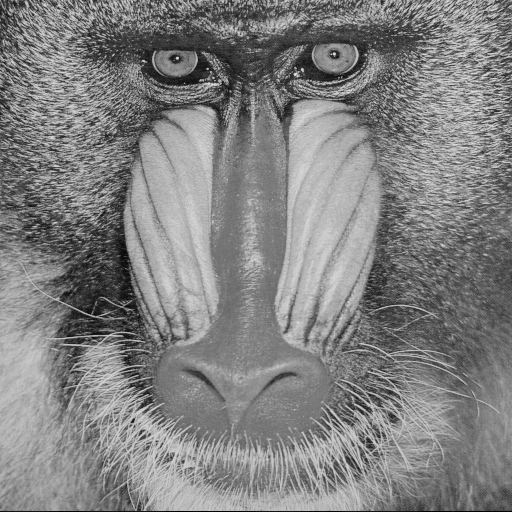
\includegraphics[width=3cm]{mandrill.png} & 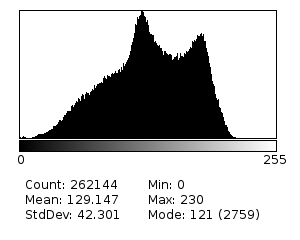
\includegraphics[width=3cm]{../histo/image/hist_mandrill.png} & 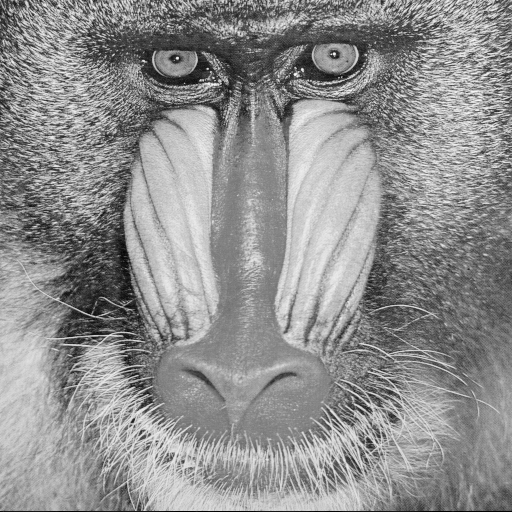
\includegraphics[width=3cm]{../res/mandrillQ1.png} & 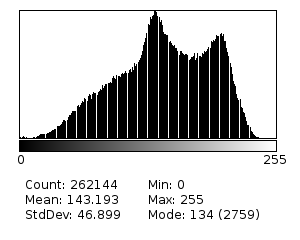
\includegraphics[width=3cm]{../histo/resultat/hist_mandrillQ1.png}\\
   \hline
   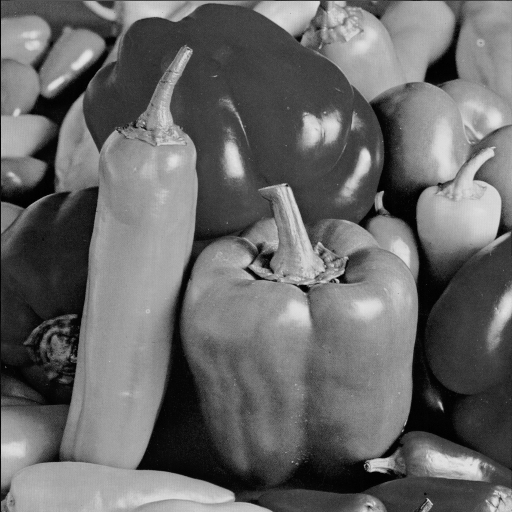
\includegraphics[width=3cm]{peppers.png} & 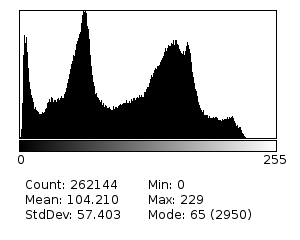
\includegraphics[width=3cm]{../histo/image/hist_peppers.png} & 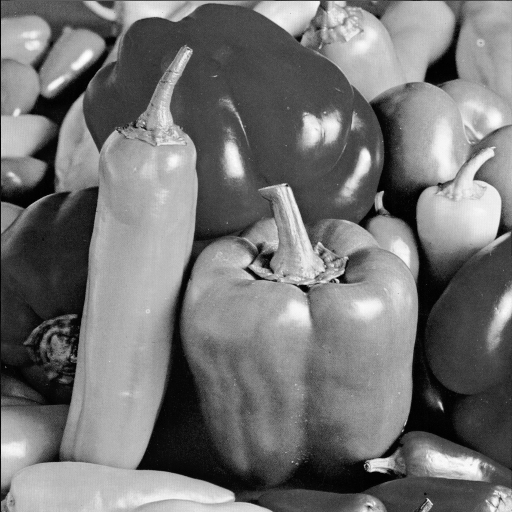
\includegraphics[width=3cm]{../res/peppersQ1.png} & 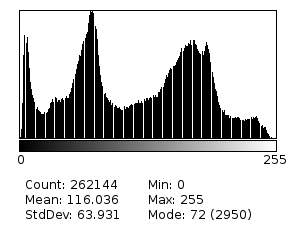
\includegraphics[width=3cm]{../histo/resultat/hist_peppersQ1.png}\\
   \hline
  \end{tabular}\\
  
  Sur ces résultats, nous pouvons voir que lorsque nous étendons l'histogramme de gris, le 
  contraste de l'image augmente. En effet, nous constatons que, dans tous les cas, l'écart-type 
  augmente, sauf lorsque la dynamique des niveaux de gris varie déjà entre 0 et 255. Nous 
  avons remarqué aussi les propriétés suivantes:
  
  \begin{itemize}
   \item Si $min>(255-max)$ alors la moyenne diminue, l'image est donc plus sombre.
   \item Si $min==(255-max)$ alors la moyenne reste identique.
   \item Si $min<(255-max)$ alors la moyenne augmente, l'image est donc plus claire.
  \end{itemize}
  
    \begin{figure}[H]
    \center
    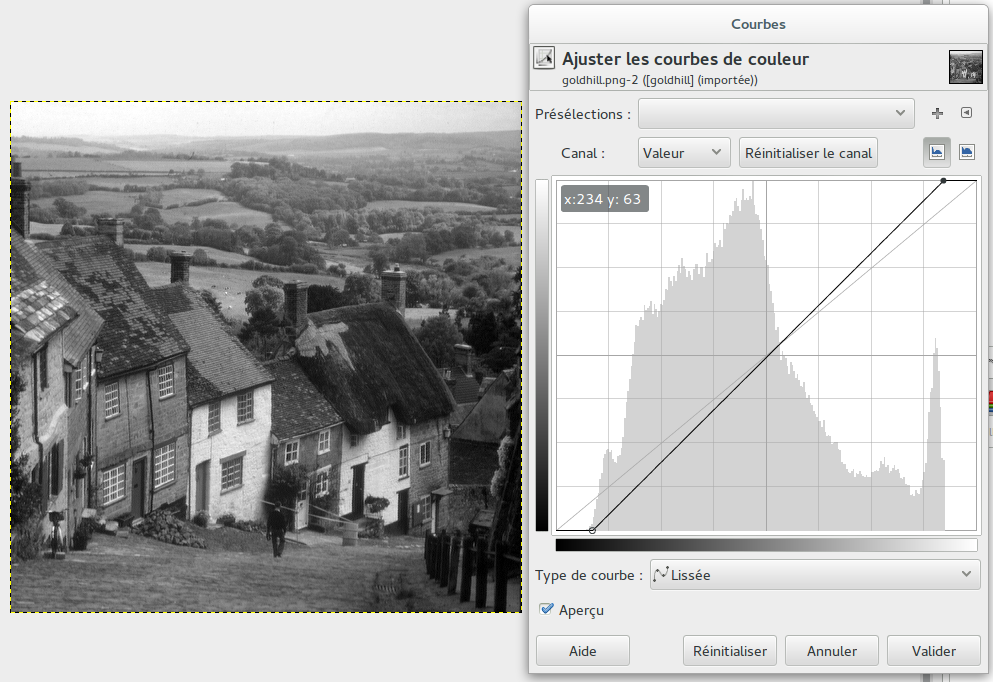
\includegraphics[width=9cm]{LUT-Q1.png}
    \caption{LUT pour étendre la dynamique sur GIMP}
  \end{figure}
  
  \section{Correction affine}
  Nous avons ensuite appliqué une correction affine du type $a+b.I(x,y)$ sur les images.
  Nous avons remarqué que plus la valeur de $a$ augmente, avec un $b$ fixé à 1, plus la 
  luminosité augmente. En effet, nous allons additionner une valeur constante à chaque 
  pixel, ce qui entraine une augmentation de $+a$ de la moyenne. Donc le nombre de pixels 
  %sombres deviendra plus clair et les pixels supérieurs à $255-a$ seront saturé à 255. 
  sombres diminuera et les pixels supérieurs à $255+a$ seront saturé à 255.
  Lorsque l'on prend une valeur négative pour $a$, l'image s'assombrit. Comme il y a 256 
  niveaux de gris, pour une image 8 bits, le nombre de pixels saturés au blanc va augmenter
  et l'écart-type va diminuer. Cependant, si nous conservons les valeurs au delà de 255 
  l'écart-type reste invariant si $b$ vaut 1.\\
  
  En revanche, la valeur de $b$ va intéragir sur le contraste de l'image, plus la valeur 
  sera grande, plus l'histogramme sera étendu. Ce coefficient influe directement sur 
  l'écart-type de l'image:
  \begin{itemize}
   \item Si $b<1$ alors l'écart-type diminue, l'image est donc moins contrastée.
   \item Si $b==1$ alors l'écart-type reste constante.
   \item Si $b>1$ alors l'écart-type augmente, l'image est donc plus contrastée.
  \end{itemize}
  \ \\
  
  \begin{tabular}{|c|c|c|}
    \hline
    Equation & Image $I'$ & Histogramme\\
    \hline
    \shortstack{Fonction sans changement \\ a=0, b=1 \\ $I'(x,y)=a+b.I(x,y)$} & 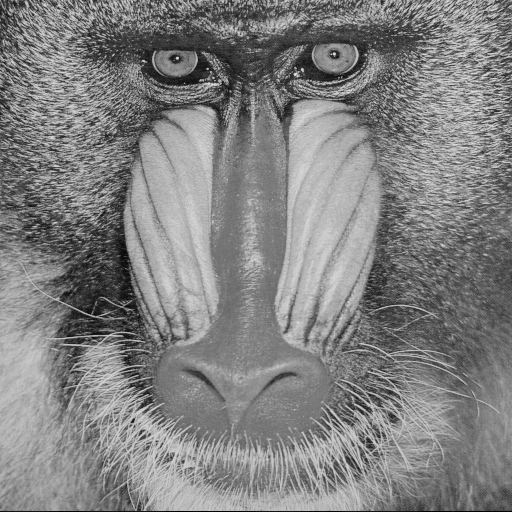
\includegraphics[width=3cm]{mandrill.png} & 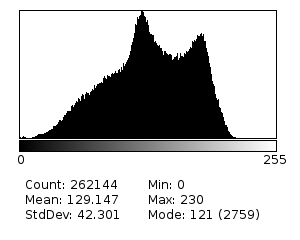
\includegraphics[width=4cm]{../histo/image/hist_mandrill.png}\\
    \hline
    \shortstack{Augmentation de la luminosité \\ a=50, b=1 \\ $I'(x,y)=a+b.I(x,y)$} & 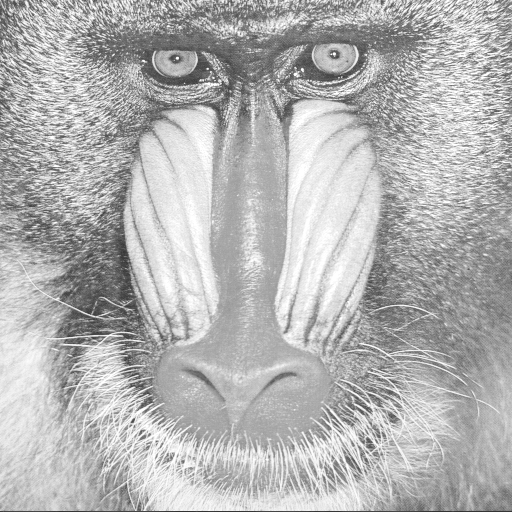
\includegraphics[width=3cm]{../res/mandrillQ2_50x1.png} & 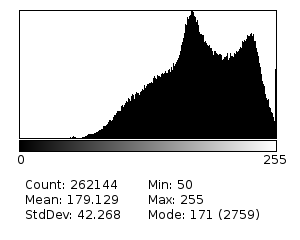
\includegraphics[width=4cm]{../histo/resultat/hist_mandrillQ2_50x1.png}\\
    \hline
    \shortstack{Augmentation de l'écart-type \\ et de la moyenne \\ a=0, b=2 \\ $I'(x,y)=a+b.I(x,y)$} & 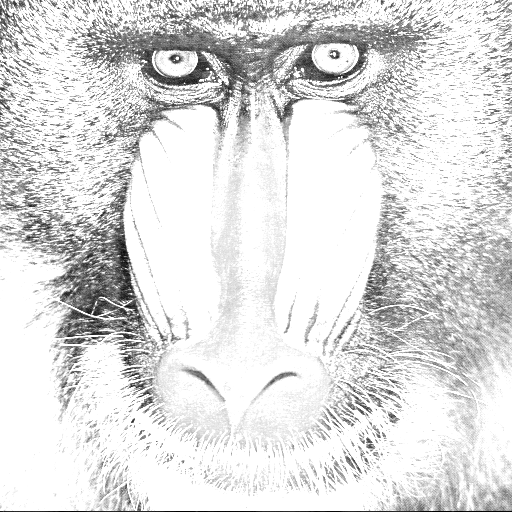
\includegraphics[width=3cm]{../res/mandrillQ2_0x2.png} & 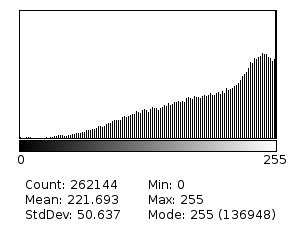
\includegraphics[width=4cm]{../histo/resultat/hist_mandrillQ2_0x2.png}\\
    \hline
    \shortstack{Fonction proximative du contraste \\ a=-64*b, b=2 \\ $I'(x,y)=a+b.I(x,y)$} & \includegraphics[width=3cm]{../res/mandrillQ2__constrast.png} & \includegraphics[width=4cm]{../histo/resultat/hist_mandrillQ2_constrast.png}\\
    \hline
  \end{tabular}
  
  
  \section{Egalisation d'histogramme}
  L'égalisation d'histrogramme est un procédé qui permet de mieux répartir les niveaux de gris sur une image.
  Pour pouvoir le calculer il nous faut d'abord récupérer l'histogramme cumulé. 
  Cet histogramme s'obtient en effectuant le calcul suivant : $hist(T)=hist(T)+hist(T-1)$. Nous obtenons donc
  un histogramme dont le nombre de pixels par niveau de gris augmente avec ce niveau. Ensuite, nous modifions la valeur de chaque pixel
  de l'image en utilisant une LUT. Lorsque nous allons modifier un pixel, nous regardons dans une table de correspondance pour 
  connaitre la nouvelle valeur du pixel que nous voulons modifier. Pour cela nous utilisons la macro suivante :
  
  \begin{lstlisting}
       ratio = 255 / (W * H);

       for (j=0; j<H; j++) {
           for (i=0; i<W; i++) {
               p = getPixel(i, j);
               new = cumule[p];
               setPixel(i, j, new * ratio);
           }
       }
  \end{lstlisting}

  Ce qui nous donne les résultats suivant : \\
  
  \begin{tabular}{|c|c|c|c|}
   \hline
   image départ & histogramme & image égalisée & histogramme\\
   \hline
   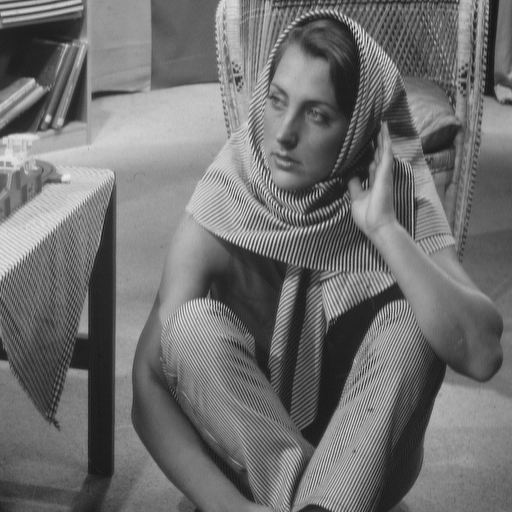
\includegraphics[width=3cm]{barb.png} & 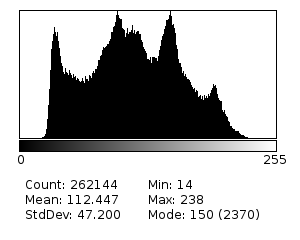
\includegraphics[width=3cm]{../histo/image/hist_barb.png} & 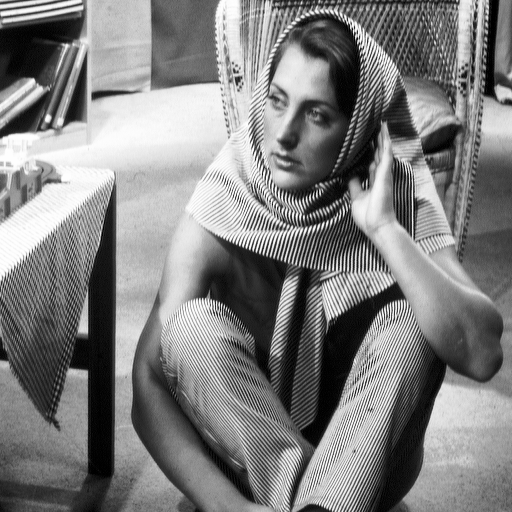
\includegraphics[width=3cm]{../res/barbQ3.png} & 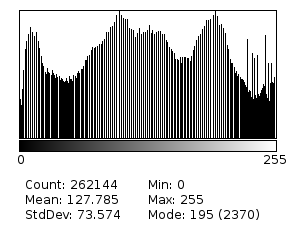
\includegraphics[width=3cm]{../histo/resultat/barbQ3.png}\\
   \hline
   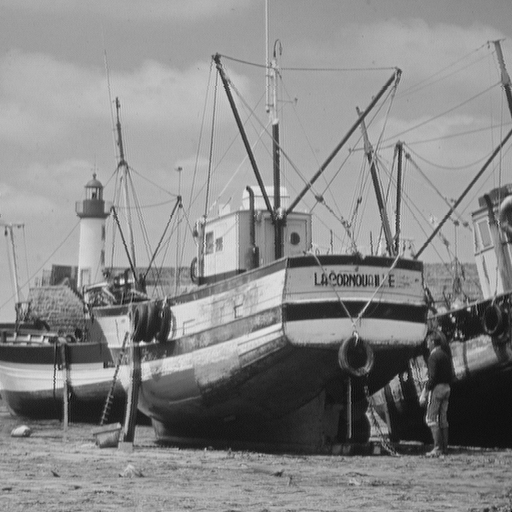
\includegraphics[width=3cm]{boat.png} & 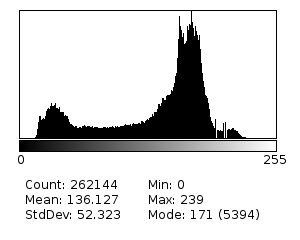
\includegraphics[width=3cm]{../histo/image/hist_boat.png} & 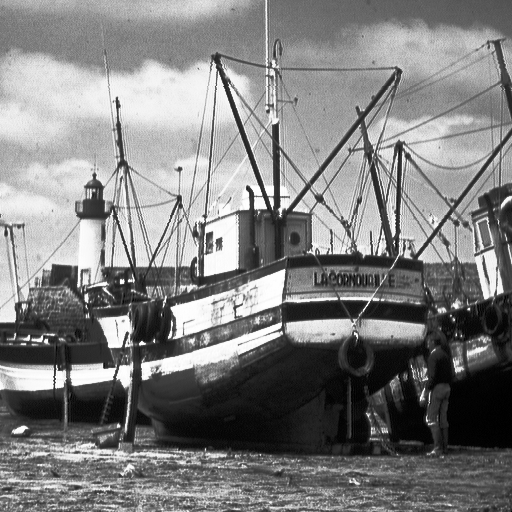
\includegraphics[width=3cm]{../res/boatQ3.png} & 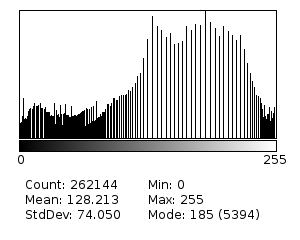
\includegraphics[width=3cm]{../histo/resultat/boatQ3.png}\\
   \hline
   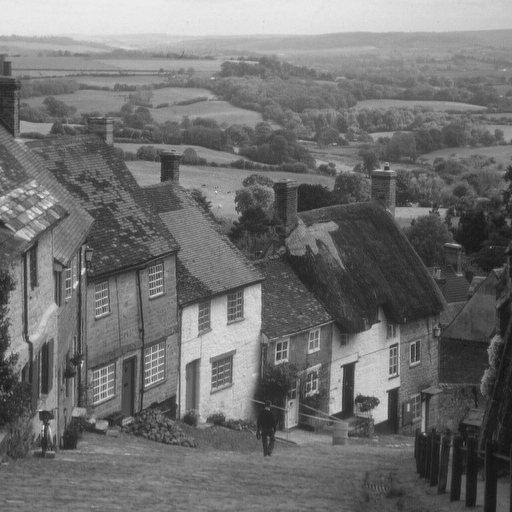
\includegraphics[width=3cm]{goldhill.png} & 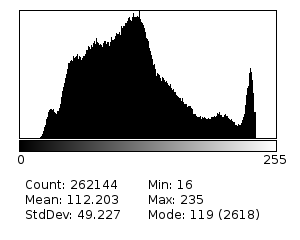
\includegraphics[width=3cm]{../histo/image/hist_goldhill.png} & 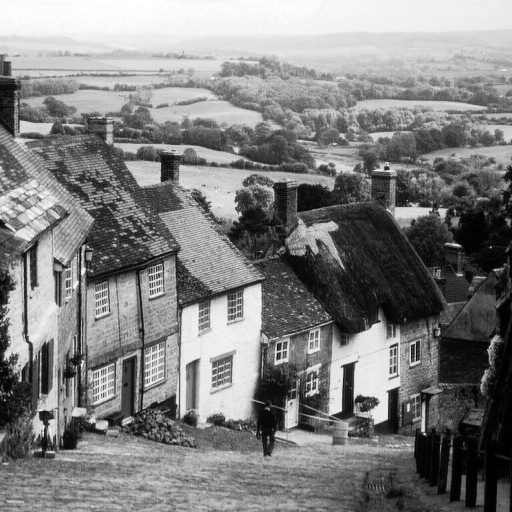
\includegraphics[width=3cm]{../res/goldhillQ3.png} & 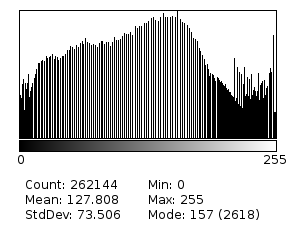
\includegraphics[width=3cm]{../histo/resultat/goldhillQ3.png}\\
   \hline
   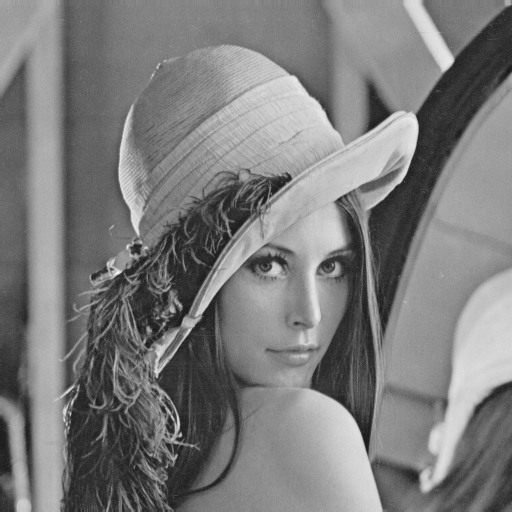
\includegraphics[width=3cm]{lena512.png} & 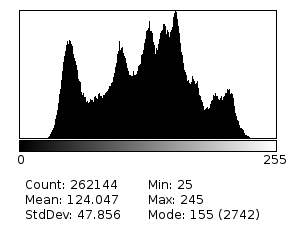
\includegraphics[width=3cm]{../histo/image/hist_lena512.png} & 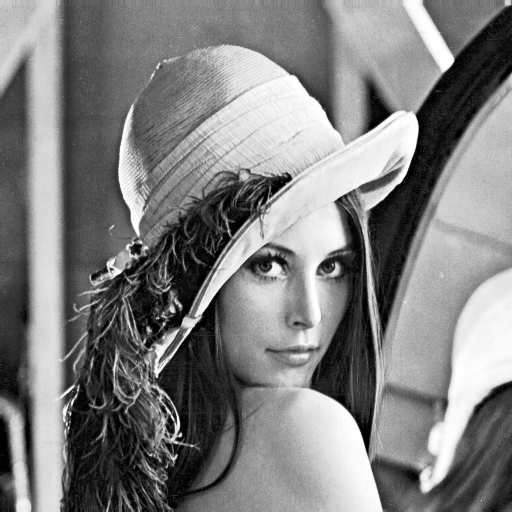
\includegraphics[width=3cm]{../res/lena512Q3.png} & 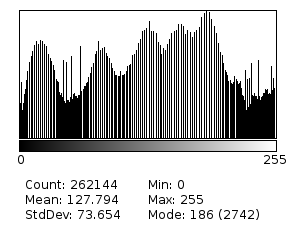
\includegraphics[width=3cm]{../histo/resultat/lena512Q3.png}\\
   \hline
   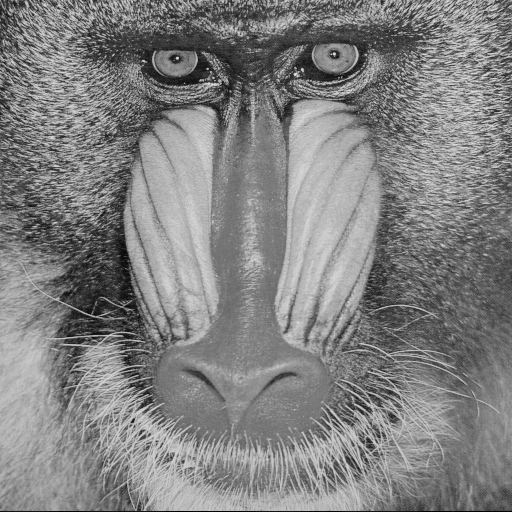
\includegraphics[width=3cm]{mandrill.png} & \includegraphics[width=3cm]{../histo/image/hist_mandrill.png} & \includegraphics[width=3cm]{../res/mandrillQ3.png} & \includegraphics[width=3cm]{../histo/resultat/mandrillQ3.png}\\
   \hline
   \includegraphics[width=3cm]{peppers.png} & \includegraphics[width=3cm]{../histo/image/hist_peppers.png} & \includegraphics[width=3cm]{../res/peppersQ3.png} & \includegraphics[width=3cm]{../histo/resultat/peppersQ3.png}\\
   \hline
  \end{tabular}\\
  
  On peut voir que l'égalisation des histogrammes n'est pas parfaite, que certains niveaux de gris ne sont pas utilisés et que d'autres 
  possèdent trop de valeurs. Obtenir un histogramme parfaitement égalisé est très difficile, voire impossible.
  \section*{Conclusion}
  Lors de ce TP, nous avons pu voir plusieurs transformations d'histogramme et leur impact sur l'image.
  \newpage
  
  \section*{Annexes}
  \begin{lstlisting}[caption=Macro d'extension d'histogramme]
  macro "setDynamiqueGray" {

    image = getImageID();

    W = getWidth();
    H = getHeight();

    min = 255;
    max = 0;

    for (j=0; j<H; j++) {
        for (i=0; i<W; i++) {

            p = getPixel(i,j);
            if ( min > p) {
                min = p;
            }

            if ( max < p) {
                max = p;
            }
         }
     }

     for (j=0; j<H; j++) {
         for (i=0; i<W; i++) {

             res = round(255 * ((getPixel(i,j) - min)/(max - min)));
             setPixel(i, j, res);
         }
     }
  }
  \end{lstlisting}
  
  \begin{lstlisting}[caption=Macro de la correction affine]
   macro "correction" {

      W = getWidth();
      H = getHeight();

      //contraste
      a = -100;
      //luminosite
      b = 2;

      for (j=0; j<H; j++) {
         for (i=0; i<W; i++) {

            res = a + b * getPixel(i,j);
            setPixel(i, j, res);
          }
      }
   }
  \end{lstlisting}

    
\end{document}  